%************************************************
\chapter{About Dorel Industries}
\label{chp:about}
%************************************************
\section{Introduction}
\centerline{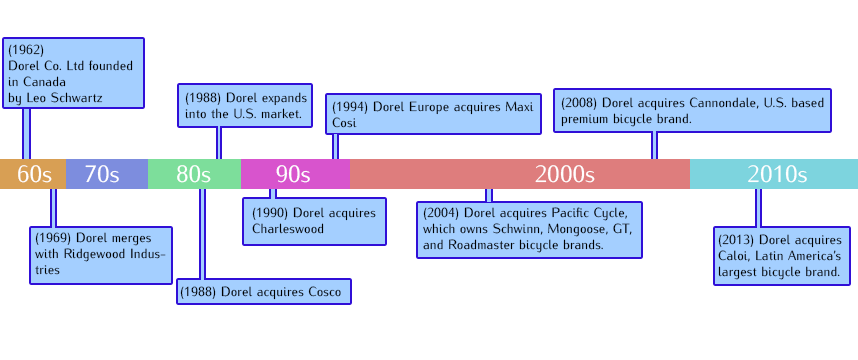
\includegraphics[scale=0.7]{Timeline}}
In 1962, Leo Schwartz founded "Dorel Co. Ltd" in Quebec, producing crib pads, mattresses, and other juvenile products.  Leo's son Martin decided to found his own company, "Ridgewood Industries", with brother-in-law Jeff Segal in 1969.  Ridgewood focused on producing ready-to-assemble furniture, and ended up finally merging with Dorel in 1987, the same year the company went public.  Since then, the company has continued to grow primarily through acquisitions, eventually branching out to the recreational and leisure markets by acquiring Schwinn and Cannondale \cite{DorelIndustries2013}.


\section{Recent Strategic Moves}\index{Recent Strategic Moves}
\begin{itemize}
  \item (2013) Dorel began a massive share buyback plan in order to raise its market value \cite{Smith2014}.
  \item (2013) The company acquired a 70\% controlling interest in Caloi (a major brazilian bicycle manufacturer).  This acquisition is intended to help Dorel expand into Latin America, as Caloi is the number one bicycle brand in the region \cite{DorelIndustries2013}.
  \item (2013) Dorel’s assembly and testing facilities located in \index{Bedford, PA}Bedford, PA are being shut down and relocated overseas in an effort to reduce expenses \cite{VoiceofAmerica2009}.
  \item (2012) Dorel began sponsoring the newly created \index{Cannondale Pro Cycling Team}"Cannondale Pro Cycling Team", in order to increase brand exposure \cite{DorelIndustries2012} .
\end{itemize}







%************************************************
\chapter{Corporate Strategy Analysis}
\label{chp:corporatestrategy}
%************************************************

\section{Business Definition}

Dorel Industries has a diverse business definition.   Dorel makes high quality furniture, juvenile and recreational products for consumers who emphasize quality and durable products.  Dorel’s technologies include ready-to-assemble furniture, high quality durable bicycles as well as safe and reliable baby products \cite{DorelIndustries2013}.

Dorel’s business is comprised of several very distinct products amongst completely unrelated markets. Dorel’s \index{Main Products}main products include furniture, bicycles and baby products.  These products relate to Dorel’s business units.   In term’s of Dorel’s target markets, the United States has traditionally been a very important market. However, due to the US economy downturn, Dorel has began focusing on extending their business internationally.  Lastly, the technology that Dorel institutes is one of outsourcing manufacture of their products, in order to be able to compete on price, specifically for their home furnishings business unit.

One of the primary issues with this business definition is that there does not appear to be much \index{Synergy}synergy among the product lines. The manufacture of the products, the products themselves, and the target markets of each product are all wholly unrelated. As part of our recommendation, Dorel would benefit from finding a way to make themselves more internally consistent.

\begin{itemize}        	
  \item Products
    \begin{itemize}
      \item Furniture
      \item Bicycles
      \item Baby products/accessories
    \end{itemize}
  \item Markets (respectively)
    \begin{itemize}     
      \item North American retail chains
      \item Mass merchant / Independent Bike Dealer (IBD) network
      \item US and International retail chains
    \end{itemize}
  \item Technology
    \begin{itemize}     
      \item Ready-to-assemble furniture
      \item High Quality products
      \item Safe and durable juvenile products
    \end{itemize}
\end{itemize}


\section{Business Unit Breakdown}
Dore’s business is comprised of 3 distinct business units; Juvenile, Home Furnishings and Recreational/Leisure.  These 3 business units drove 2012 revenue of \$2.49 Billion, as well as \$583 Million in gross profit. A breakdown of each business unit follows.

\subsection{Juvenile}
The \index{Juvenile}Juvenile business unit is focused on the manufacture and import of high quality, safe and fashionable juvenile products.  These products include car seats, strollers, high chairs, etc.  Products are provided under their own brand names, as well as house brand names for their customers. This segment produced 2012 revenues of \$1.04 Million, which equates to 42\% of the business. This segment produced \$287 Million in \index{Gross Profit}gross profit which was 49\% of Dorel’s total gross profit.

Dorel is focusing on growing this segment in Latin America, where the retail environment is beginning to prosper and birthrates in this region are an incline. Dorel has also made very recent \index{Acquisitions}{acquisitions for this segment to expand its breadth of offering as well as introduction to new international channels.

\subsection{Recreational/Leisure}
The \index{Recreational/Leisure}Recreation/Leisure business is comprised of premium/mass market bicycles, jogging strollers, ride-on toys as well as branded performance apparel.  This segment has a focus on international markets, with 50\% of sales coming from the Asia-Pacific region (US accounts or 12\%). This segment accounted for 37\% of Dorel’s 2012 revenue, or \$928 Million, with gross profit at \$233 Million.

Dorel is focused on making this segment the premier bicycle business in the market. in 2012, \index{Expenses}selling expenses for this business unit increased 13\%, which leadership attributed to \index{Marketing}marketing efforts to enrich this segment’s brands.

\subsection{Home Furnishings}
\index{Home Furnishings}The Home Furnishings business focuses on ready-to-assemble furniture, step stools, futons and imported home entertainment furniture.  The primary focus for this segment is North American markets, which is evident since Dorel has five distinct segments within this business unit. This segment drove 21 percent of Dorel’s 2012 revenue with \$521 million, as well as 11% of gross profit with \$62 million

This segment is the \index{Cash Cow}cash cow for Dorel.  However, with this segment’s focus being on the North American market, home-related market, this segment has suffered a bit with the \index{US Economy}US economy.  Recenty, Dorel moved more of its manufacturing overseas, which should help with this segment’s ability to compete on price in their mass retail chains.

\begin{table}[h]
    \begin{tabular}{lllllllllll}
    {\bf \underline{Unit}}                 & {\bf \underline{Total Sales}}    & {\bf \underline{\%}}  & {\bf \underline{Gross Profit}} & {\bf \underline{\%}}\\
    Juvenile             & \$1,040,765,000 & 42\% & \$287,658,000 & 49\% \\
    Home Furnishings     & \$521,523,000  & 21\% & \$62,552,000 & 11\% \\
    Recreational/Leisure & \$928,422,000  & 37\% & \$233,437,000 & 40\% \\
    \end{tabular}
\end{table}

\begin{table}[h]
    \begin{tabular}{lllllllllll}
    {\bf \underline{Unit}}             &  {\bf \underline{Operating Profit}} & {\bf \underline{\%}}  & {\bf \underline{Unit Strength}} & {\bf \underline{Industry Potential}} \\
    Juvenile             & \$73,313,000     & 43\% & 3 & 4 \\
    Home Furnishings     & \$25,593,000     & 15\% & 1 & 2 \\
    Recreational/Leisure  & \$71,958,000     & 42\% & 4 & 2 \\
    \end{tabular}
\end{table}
%----------------------------------------------------------
%************************************************
\section{Modified BCG}
\label{chp:bcg}
%************************************************
\centerline{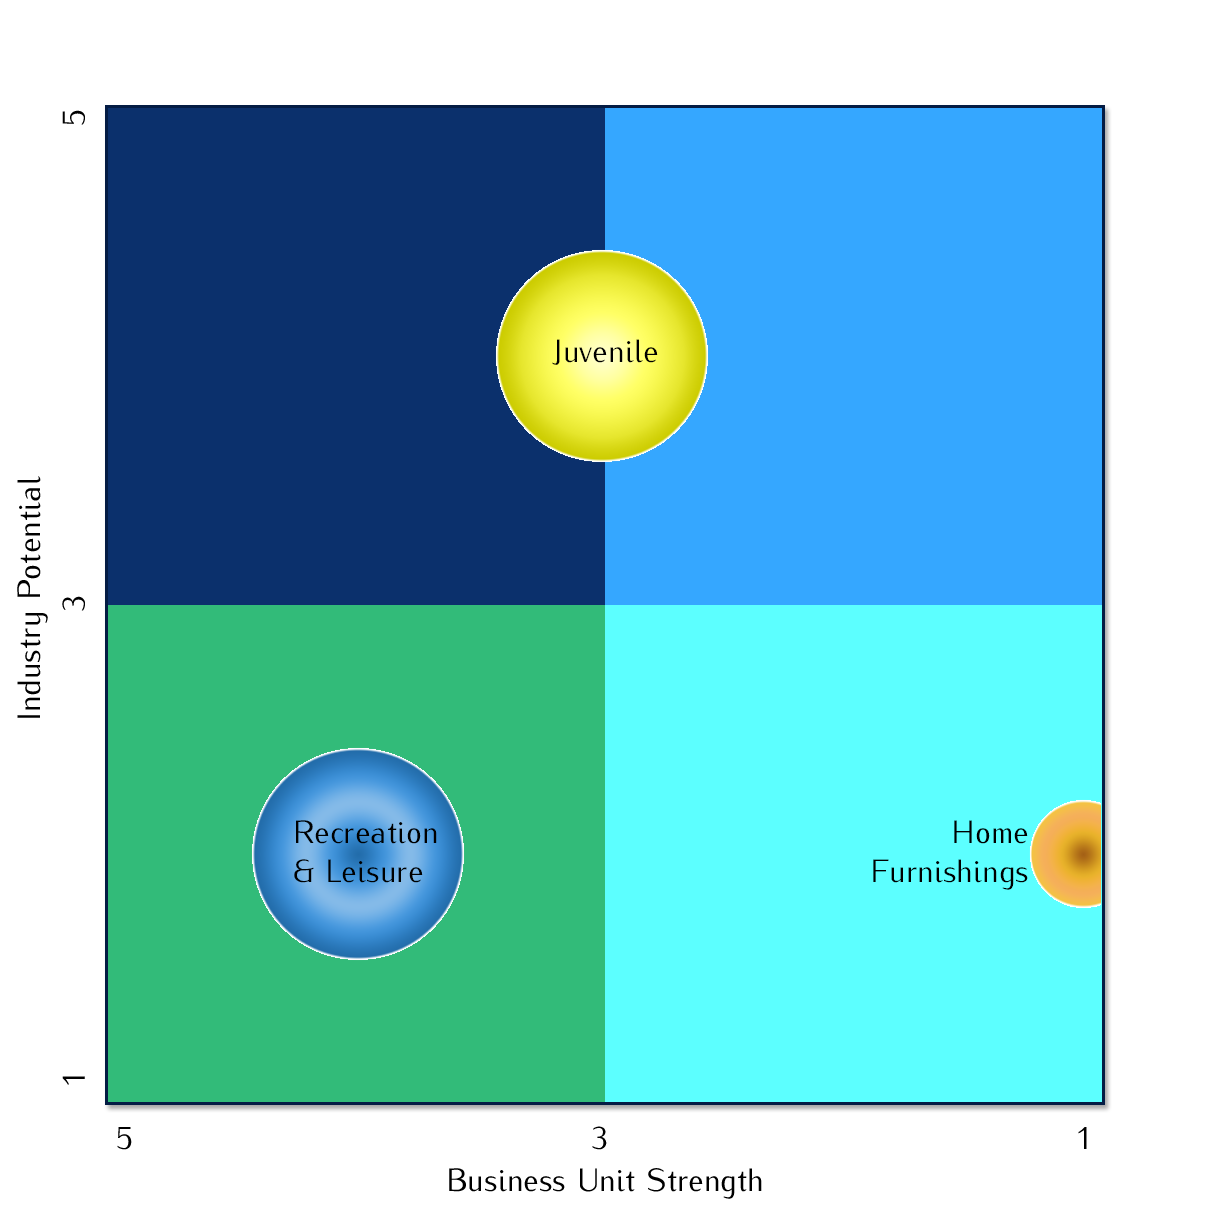
\includegraphics[scale=0.5]{BCG}}
\subsection{BCG Analysis}
This BCG graph illustrates some of Dorel's current issues.  Currently the company has built a substantial cash cow in the recreational and leisure unit, which is generating on average 42\% of the annual operating profit.  However, furnishings remains a dog, bringing in only about 15\% of the company's revenue, with little sign future industry potential.  The Juvenile SBU is hovering between a questin mark and star, and we believe with our recommendations, has the potential to bring Dorel the most revenue in the future.
%---------------------------------------------------------------

%************************************************
\section{Five Tests}
\label{chp:tests}
%************************************************
\paragraph{NOTE:}We have decided to rate the company on a scale of 1-5 for each of the \index{Five Tests}five tests based on its current standing, as well as the rating we believe it can achieve with improved guidance on its corporate strategy.



\subsection{Vision}
At present, Dorel scores an abysmal one out of five on \index{Vision}vision.  The company has over extended into several very unrelated markets, does not seem to have any type of BHAG, and is relying on acquisitions instead of innovation in order to gain market share.  When the company was founded in 1962, it was built on three \index{Core Values}core principles: \index{Safety}safety, \index{Quality}quality, and \index{Value}value.  In direct contrast to those pillars, in recent years Dorel has in an attempt to reduce cost has compromised on quality and safety. This resulted in several recalls, including over half a million baby cribs in 2010 after several injury reports and even one death \cite{Commission2010}.  In the recreation \& leisure unit, Dorel has taken a brand \index{Schwinn}(Schwinn) once known for high quality and reduced its brand recognition to mediocre at best.  It is currently unclear what vision Dorel’s management is even aiming for, as aside from acquiring new brands and outsourcing overseas to reduce costs, there is very little on the horizon for the company.  

\subsection{Internal Consistency}
Dorel’s \index{Internal Consistency}internal consistency suffers from the same issues as it’s vision, in that it currently serves three very different markets.  However, each niche consists of a variety of brands that are consistent and complementary to each other.  As an example, Dorel’s Recreational/Leisure division has acquired several major bicycle brands, including Mongoose, Schwinn, and GT.  While overall the internal consistency and fit within Dorel might not be strong, because of the strength within each unit we have given Dorel a three on consistency.

\subsection{External Fit}
In terms of \index{External Fit} external fit and consistency, we gave Dorel a three out of five.  Because Dorel has already established itself in three different segments, and because of the amount of revenue currently coming in with its cash cows (Furnishings/Juvenile), Dorel has the capital and experience to dominate any of the three markets it is in, but only if it can return to the core values that the company was founded on.

\subsection{Corporate Advantage}
In the \index{Corporate Advantage}corporate advantage test we scored Dorel a two out of five. Although the company is able to leverage their supply chain and reduce costs for all three business units, aside from the distribution network, there is very little corporate advantage.  Because each of the divisions are in completely unrelated markets, research and development cannot be leveraged across business units.

\subsection{Feasiblity}
In the \index{Feasibility}Feasibility test we scored Dorel a two out of 5. This is based upon a current lack of envisioned future an leadership.  However, Dorel has a high potential for improving the in juvenile products, and have recently made investments in that direction. The juvenile market is growing at 3 percent annually, and Dorel is currently the market leader for North America. 

%************************************************
\section{Financial Metrics}
\label{chp:financials}
%************************************************
\subsubsection{10 Year Overview}
\centerline{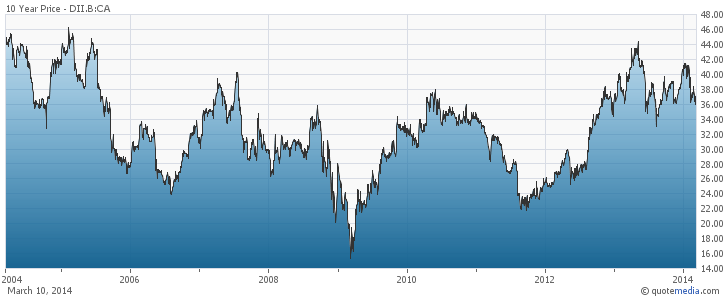
\includegraphics[scale=0.5]{5year}}
Over the past 10 years, Dorel has struggled to return to it's high of \$46 per share in 2005, and is currently trading at about \$37 per share.   

\subsubsection{Last 2 Years}
\centerline{\includegraphics[scale=0.8]{Stocks2Year}}
\index{Stock Price}Recently however, Dorel has performed fairly well, outpacing indices and maintaining high growth for the last two years. \cite{YahooFinance2014}.

\subsubsection{Current Year (2014)}
\centerline{\includegraphics[scale=0.8]{Stocks1Year}}
However, after a very weak \index{Q4 Performance}Q4 performance at the end of 2013, Dorel's \index{Current Stock Price}stock price has fallen substantially this year \cite{YahooFinance2014}.

%************************************************
\chapter{Competitive Strategy Analysis}
%************************************************

\section{Juvenile Industry Definition}
\subsection{The Product \& Market Scope}
The juvenile industry is defined by the JPMA (Juvenile Products Manufacturers Association) as any products targeted for the prenatal to preschool age groups.  Some of the primary products in the market include car seats, strollers, high chairs, infant home safety equipment, and cribs.  Geographically Dorel is already in several international markets, with a strong presence in North America, Europe, and Latin America.

\section{The Who and What}
\subsection{Suppliers}
The suppliers in the Juvenile market primarily relate to raw meterials (Plastics, wood, paint, fabric etc.) and labor (Domestic \& Overseas), with much of the physical work outsourced.  Because of this, the suppliers have low leverage, as Dorel and other Juvenile product manufacturers have low switching costs to other suppliers.

\subsection{Potential Entrants}
There are few possible new entrants to the Juvenile market, aside from foreign competitors, and private label retailers.  Due to high amounts of government regulation and safety requirements, the barrier to new entrants is high.

\subsection{Competitors}
Current competitors to Dorel include Safety 1st, Graco, EvenFlo, Huggies, and Pampers.  Dorel is currently number one in North America and has the potential to dominate other markets.

\subsection{Substitutes}
There are few physical substitutes in the Juvenile market, as there is no real alternative to products such as car seats, cribs, etc.  However, as Porter's article mentioned, there can be other more subtle substitutes.  The main substitute is most likely the used product market, as many parents choose to instead purchase previously used items.

\section{Industry Environment and Dynamics}
\subsection{Customer Ratio}
Presently the customer ratio is in favor of competitors in the juvenile industry, as most parents at some point will require at least some of the products.  However, the switching costs are extremely low, with companies competing primarily on price point.  If Dorel follows our recommendation of quality over quantity however, we hope to become a differentiated market player that commands a higher value than competitors.
\subsection{Macro-environmental Factors (PESTLE Analysis)}
Listed below are some of the major macro-environmental factors impacting the juvenile market, analy:
\subsubsection{Political Trends}
As mentioned previously, high amounts of governmenet regulation are actualy a positive in the juvenile market, as it raises the barrier to entry for newcomers, as well as helping to ensure products meet a minimum level of safety.
\subsubsection{Economic Growth and Stability}
Economically, retail sales continue to slowly increase, and families are beginning to have more discretionary income.  However, the recent economic downturn a few years ago could be making customers gun-shy of spending.  Another negative factor is the lifecycle of products is increasing, with services such as Craigslist and Ebay increasing the second-hand market.
\subsubsection{Sociocultural Trends}
In most first world countries, there is a high emphasis in society for taking care of young children, which positively impacts the juvenile market.  Conversely however, birth rates are dropping, decreasing the market size.  Because of this, many competitors in the juvenile market including Dorel, are expanding into areas that have the highest birth rates (Latin America, Asia, etc.).
\subsubsection{Technological Advancements}
There have been few technological advancements in the juvenile market, aside from innovations in the manufacturing process that have allowed for lower production costs.  The negative side to this is a lack of ability to differentiate from competitors.
\subsubsection{Legal and Regulatory Issues}
From a legal standpoint, laws requiring child safety devices (car seats) has greatly increased the juvenile market.  However, because of the nature of the products, there is a very high threat of litigation if the product fails to protect the child.

\subsubsection{Ecological Environment Trends}
Ecologically there have been few trends in recent years, aside from a focus on eco-friendly manufacturing.  This has led to some marketing being directed at "Green" products, but has had littie impact on the juvenile market.	

\section{Key Success Factors}
\centerline{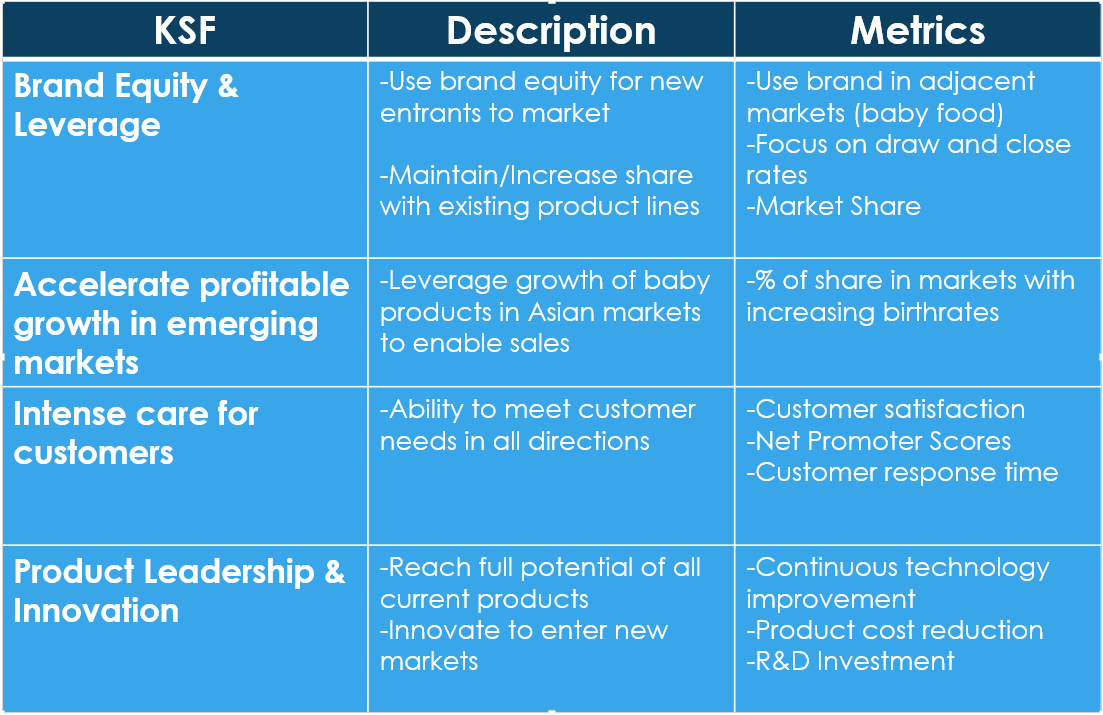
\includegraphics[scale=0.5]{KSF}}
We feel that factors mentioned above are vital in getting Dorel back on track to become a quality manufacturer of not just Juvenile products, but for being successful with all three SBUs.  

%************************************************
\chapter{Recommendations}
\label{chp:recommendations}
\index{Recommendations}
%************************************************

\section{Walk the Line with Quality!}
\index{Quality over Quantity}We believe that in order to be successful, Dorel must return to its original core values of quality, safety, and value.  Currently, the company has drifted to a philosophy of cutting costs wherever possible, and only measuring success based on the current profit margin \cite{BRAINStaff2012}.  If Dorel continues down this path, it will lead to competing solely on price point, ironically still dropping \index{Profit Margins}profit margins.  We propose alternatively, that Dorel budget extensively for improving quality, which will in turn dramatically improve safety as well as increasing the \index{Value}value of its products.  This will make it easier to market those products, as well as increasing \index{Profit Margins}profit margins through \index{Brand Recognition}brand recognition. 

In order for Dorel to become a producer of premium products, one of the first steps we would like to see is a large increase in the R\&D budget, with the company ideally becoming differentiated for same reasons as Apple.  In combination with this strategy, we also believe the company should strongly push into online markets.  This will do several things to improve Dorel, including reducing consumer purchasing power (as retailers like Walmart will no longer be able to strong-arm Dorel).  It will also create a test market for new innovative products that will require very little inventory liability.  We envision Dorel testing it's newest products online first, and if successful, selling them at retailers as well.  

If these changes are implemented, we feel that Dorel can become known as the number one manufacturer of premium products in the juvenile, recreational/leisure, and possibly home furnishings markets.  This will create a higher margin potential, especially if they are able to incorporate direct to consumer sales through the online portal, as well as from much-needed differentiation.  In the next 5 years, we believe Dorel should focus more on building brand loyalty than on acquisitions.  By doing so, we expect the juvenile unit to become a star.  Here is a 





%************************************************
\chapter{Appendix}
%************************************************

\subsection{Revenue}
\centerline{\includegraphics[scale=0.5]{Revenue}}
\paragraph{Revenue \& Net Income}By looking at data from the last 8 quarters, we have determined that annual revenue has fallen by 6 million in 2013 as compared to 2012, and \index{Net Income}net income has decreased as well by 44\% (Comparing 2013 Q3 earnings of \$11.1 million vs. 2012 Q3 earnings of \$20 million) 
\\[1\baselineskip]

\centerline{\includegraphics[scale=0.5]{RevenueBySegment}}
\paragraph{Revenue by Unit}In 2012, revenue decreased by 1\% in home furnishings, and increased by 1\% in recreational/lesiure
\\[1\baselineskip]

\centerline{\includegraphics[scale=0.5]{RevenueByGeography}}
\paragraph{Revenue by Geographical Distribution}\index{Revenue by Geographical Distribution}Revenue has been consistenly decreasing in the United States, while slowly increasing in other countries (Dorel is currently pushing its recreational/leisure unit into several new markets in Latin America, and is also has some highly successful brands in India) \cite{BRAINStaff2013}.


\subsection {Financial Performance by Unit}
\centerline{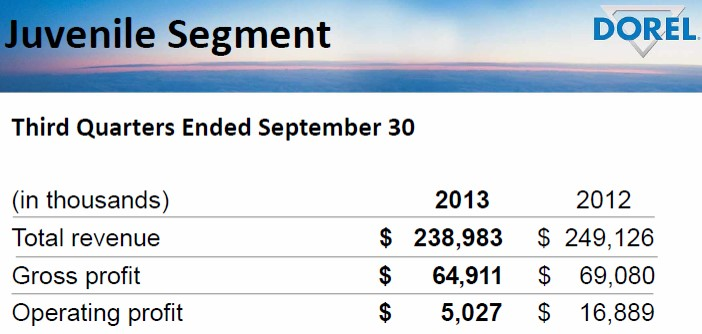
\includegraphics[scale=0.7]{juvenile}}
\centerline{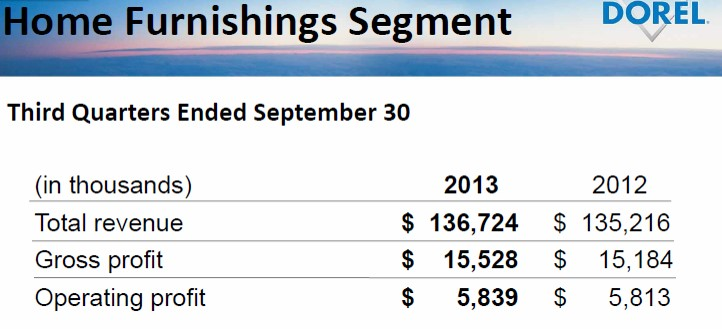
\includegraphics[scale=0.7]{furnishings}}
\centerline{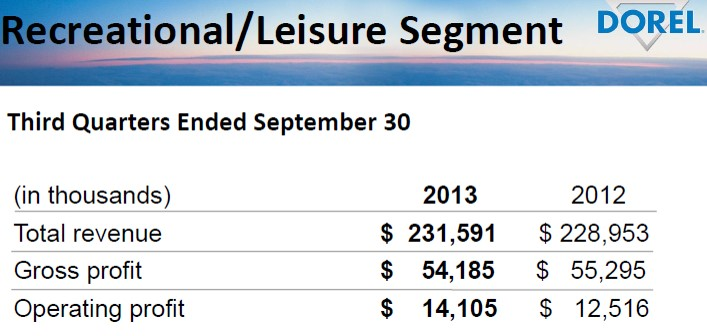
\includegraphics[scale=0.7]{recreational}}

%************************************************
\section{Balanced Scorecard}
\label{chp:scorecard}
%************************************************
\centerline{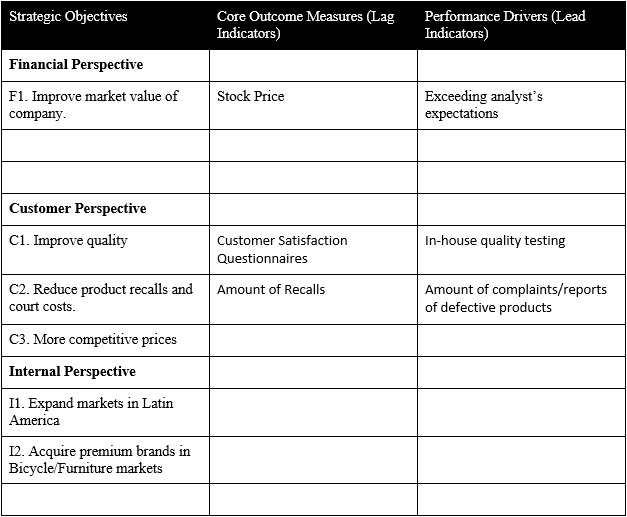
\includegraphics[scale=0.7]{scorecard}}

%************************************************
\section{SWOT Analysis}
\label{chp:swot}
%************************************************
\centerline{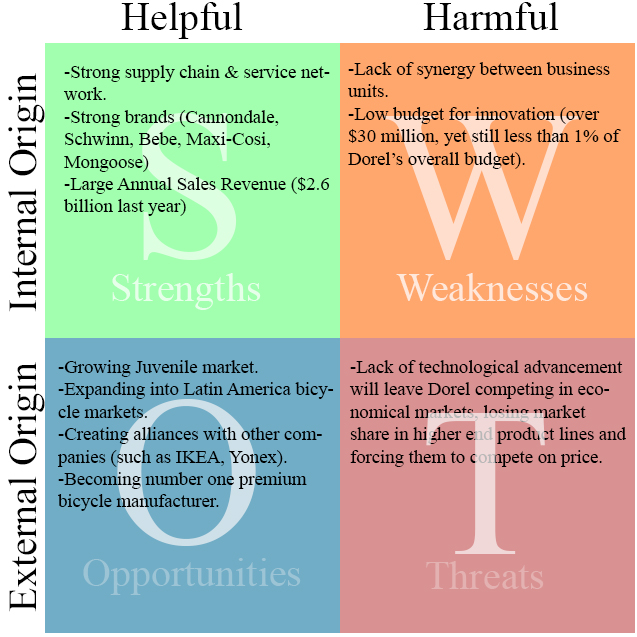
\includegraphics[scale=0.5]{SWOT}\index{SWOT}}